\documentclass[12pt, a4paper]{article}
\usepackage[margin=2.5cm]{geometry}
\usepackage[hidelinks]{hyperref}
\usepackage{tabularx}
\usepackage{enumitem}
\usepackage{booktabs}
\usepackage{cite}
\usepackage{graphicx} % Required for inserting images
\usepackage{tikz}
\usetikzlibrary{shapes.geometric, positioning}

\setlength{\parindent}{0pt}
\setlength{\parskip}{0.5em}

\begin{document}

\begin{center}
\textbf{\Large ENN595-1 Project Students Semester Two 2026} \\
\vspace{0.3cm}
\textbf{\Large Investigation via the Engineering Literature} \\
\vspace{0.3cm}
\textbf{\Large Assessment 1A} \\
\vspace{0.3cm}
\end{center}

\vspace{0.5cm}
\noindent Student Name: Joshua Hecke \\
\vspace{0.2cm}

\noindent Student No\# : n11585382 \\
\vspace{0.2cm}

\noindent Research Topic Title: Investigation of Primitive-Space Scene Change Detection in Underwater 3D Gaussian Splatting Models \\
\vspace{0.2cm}

\noindent Project Supervisor: Niko Sünderhauf \\
\vspace{0.5cm}

\section*{Assessment Tasks}
\begin{enumerate}
    \item Draw and label a concept map of your research topic;
    \item Translate those key concepts into a search statement;
    \item Search for relevant engineering literature in a library database;
    \item Identify authoritative, reputable and reliable information sources relevant to your research topic;
    \item Submit a summary analysis and evaluation of three (3) key references;
    \item Locate three (3) published authorities (acknowledged experts) in your field of research;
    \item Identity, categorize and synthesise trends and directions found in the literature;
    \item Explain what impact the literature findings have had on the design of your project;
    \item Compile a reference list of the most useful literature on your topic.
\end{enumerate}
This document has been prepared using the provided template on Canvas. It contains identical sections and headings to the template.


\section*{Concept Map : Draw and label a graphical outline view of your research question.}

\begin{center}
\resizebox{\linewidth}{!}{
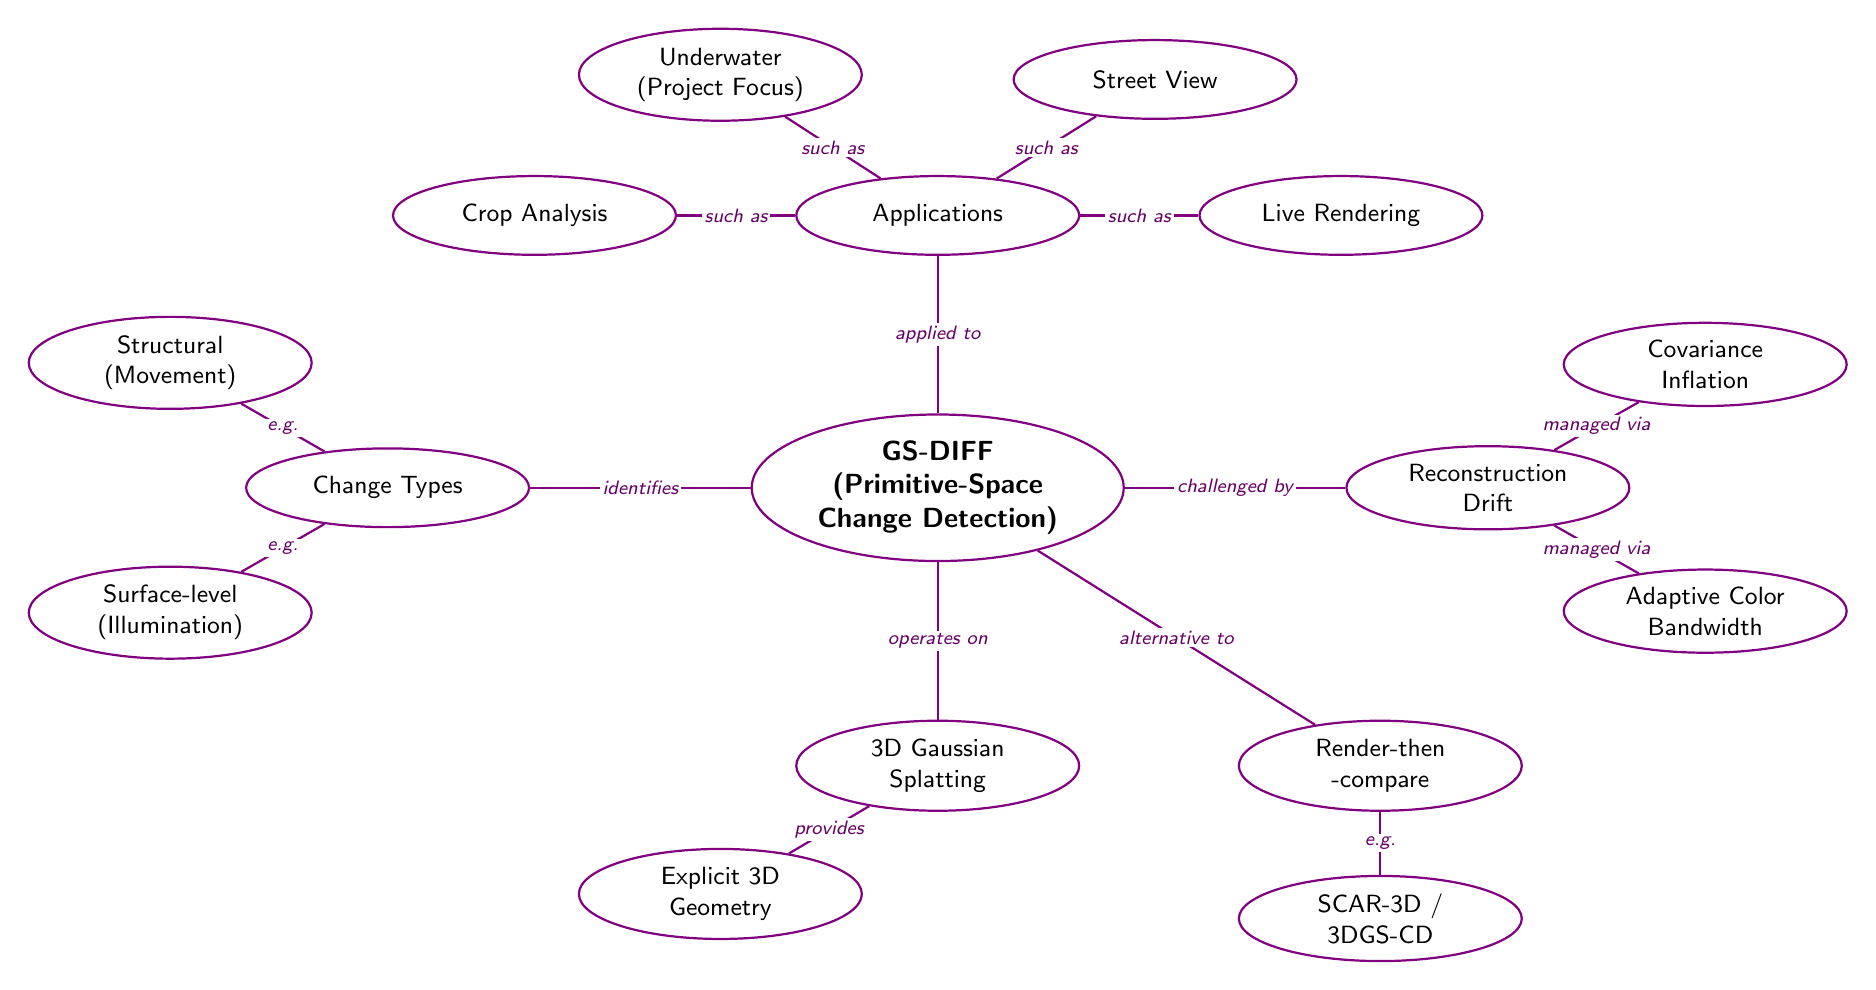
\begin{tikzpicture}[
    node distance=1cm and 2cm,
    every node/.style={align=center, font=\sffamily\small},
    concept/.style={ellipse, draw=violet, thick, inner sep=2pt, text width=2.4cm, minimum height=1cm},
    main concept/.style={concept, font=\sffamily\bfseries\normalsize, text width=3.2cm, minimum height=1.3cm},
    edge text/.style={fill=white, inner sep=1pt, font=\sffamily\scriptsize\itshape, text=violet!80!black}
]

% Nodes
\node[main concept] (gsdiff) {GS-DIFF\\(Primitive-Space Change Detection)};

% Top: Applications
\node[concept, above=2cm of gsdiff] (apps) {Applications};
\node[concept, above left=1cm and 0.2cm of apps] (underwater) {Underwater\\(Project Focus)};
\node[concept, above right=1cm and 0.2cm of apps] (street) {Street View};
\node[concept, left=1.5cm of apps] (crop) {Crop Analysis};
\node[concept, right=1.5cm of apps] (live) {Live Rendering};

% Bottom: 3D Gaussian Splatting & Alternatives
\node[concept, below=2cm of gsdiff] (3dgs) {3D Gaussian\\Splatting};
\node[concept, below left=0.8cm and 0.2cm of 3dgs] (explicit) {Explicit 3D\\Geometry};
\node[concept, right=2cm of 3dgs] (render) {Render-then\\-compare};
\node[concept, below=0.8cm of render] (scar) {SCAR-3D /\\3DGS-CD};

% Left: Change Types
\node[concept, left=2.8cm of gsdiff] (detects) {Change Types};
\node[concept, above left=0.8cm and 0.2cm of detects] (structural) {Structural\\(Movement)};
\node[concept, below left=0.8cm and 0.2cm of detects] (surface) {Surface-level\\(Illumination)};

% Right: Challenges
\node[concept, right=2.8cm of gsdiff] (drift) {Reconstruction\\Drift};
\node[concept, above right=0.8cm and 0.2cm of drift] (covariance) {Covariance\\Inflation};
\node[concept, below right=0.8cm and 0.2cm of drift] (color) {Adaptive Color\\Bandwidth};

% Edges
\draw[violet, thick] (gsdiff) -- node[edge text] {applied to} (apps);
\draw[violet, thick] (apps) -- node[edge text] {such as} (underwater);
\draw[violet, thick] (apps) -- node[edge text] {such as} (street);
\draw[violet, thick] (apps) -- node[edge text] {such as} (crop);
\draw[violet, thick] (apps) -- node[edge text] {such as} (live);

\draw[violet, thick] (gsdiff) -- node[edge text] {identifies} (detects);
\draw[violet, thick] (detects) -- node[edge text] {e.g.} (structural);
\draw[violet, thick] (detects) -- node[edge text] {e.g.} (surface);

\draw[violet, thick] (gsdiff) -- node[edge text] {challenged by} (drift);
\draw[violet, thick] (drift) -- node[edge text] {managed via} (covariance);
\draw[violet, thick] (drift) -- node[edge text] {managed via} (color);

\draw[violet, thick] (gsdiff) -- node[edge text] {operates on} (3dgs);
\draw[violet, thick] (3dgs) -- node[edge text] {provides} (explicit);
\draw[violet, thick] (gsdiff) -- node[edge text] {alternative to} (render);
\draw[violet, thick] (render) -- node[edge text] {e.g.} (scar);

\end{tikzpicture}
}
\end{center}

\textbf{Overall Project Objective:} To research and evaluate the application of primitive-space scene change detection (specifically GS-DIFF) on 3D Gaussian Splatting models reconstructed from underwater environments. 
\\\textbf{Questions to be investigated:}
    \begin{itemize}
        \item 1. Can the primitive-space comparison method (GS-DIFF) handle the specific geometric and photometric drift inherent in underwater 3DGS reconstructions?
        \item 2. Can the integration of Surface-Aligned Gaussian Splatting (SuGaR) into the GS-DIFF pipeline improve scene change detection accuracy on complex underwater geometry by enforcing structural regularization and mitigating reconstruction noise?
    \end{itemize}
\textbf{Scope:} Focus on newly proposed 3D Gaussian Splatting methods designed for underwater environments (such as WaterSplatting, SeaSplat, and Aqua-Splat) and the application of scene change detection within these complex marine models.
\vspace{3cm}




\section*{Now take the terms and phrases from your concept map to develop and refine a search strategy.}
\begin{table}[h]
\centering
\renewcommand{\arraystretch}{1.5}
\begin{tabular}{|>{\centering\arraybackslash}p{3.5cm}|c|>{\centering\arraybackslash}p{3.5cm}|c|>{\centering\arraybackslash}p{3.5cm}|}
\hline
1st Concept & AND & 2nd Concept & AND & 3rd Concept \\
\hline
3D Gaussian Splatting & & Change Detection & & Applications \& Environments \\[1.5cm]
\hline
\end{tabular}
\end{table}


\begin{table}[h]
\centering
\renewcommand{\arraystretch}{1.5}
\begin{tabular}{|c|>{\centering\arraybackslash}p{3.5cm}|c|>{\centering\arraybackslash}p{3.5cm}|c|>{\centering\arraybackslash}p{3.5cm}|c|}
\hline
OR & Synonyms & AND & Synonyms & AND & Synonyms & OR \\
\hline
 & 3DGS, Explicit Geometry, SuGaR & & GS-DIFF, Render-then-compare & & Underwater, Street View, Crop Analysis & \\[1.5cm]
\hline
\end{tabular}
\end{table}

\begin{center}
\fbox{\parbox{0.8\textwidth}{
\vspace{0.2cm}
\centering splat*, geometr*, detect*, compar*, underwat*, crop*, street*
\vspace{0.2cm}
}}
\end{center}

\begin{center}
\fbox{\parbox{0.9\textwidth}{
\vspace{0.2cm}
\centering
("Abstract":"3D Gaussian Splatting" OR "Abstract":"3DGS" OR "Abstract":"Explicit Geometry" OR "Abstract":"SuGaR") \\
AND ("Abstract":"change detection" OR "Abstract":"GS-DIFF" OR "Abstract":"render-then-compare") \\
AND ("All Metadata":underwater OR "All Metadata":"street view" OR "All Metadata":"crop analysis")
\vspace{0.2cm}
}}
\end{center}
\vspace{0.2cm}
\noindent\textbf{Search Strategy Justification:} The search leverages logical Boolean operators (AND/OR) to combine the three key concepts effectively. Truncation (e.g., splat*, geometr*) captures grammatical variants. Crucially, field restrictions (limiting terms to "Abstract" and "All Metadata") are employed to focus the results strictly on papers where these concepts are the primary focus of the research, thereby drastically reducing false positives and increasing search efficacy.



\section*{Search for relevant engineering literature in a library database.}

\textbf{Database Name:} IEEE Xplore \\
\textbf{Database Platform:} IEEE \\

\textbf{Comment on the scope and justification:} IEEE Xplore was selected as the primary database because it is the premier, most authoritative repository for engineering and computer science literature. It provides exclusive access to high-impact proceedings from the IEEE Robotics and Automation Society (e.g., ICRA, IROS, RA-L) and the IEEE Computer Society (e.g., CVPR, ICCV). Because underwater 3D Gaussian Splatting and primitive-space change detection are extremely recent, cutting-edge developments, they appear almost exclusively in these rapid-publication conferences and letters rather than traditional long-form journals. Therefore, IEEE Xplore is highly cogent and the most useful database to capture the true state-of-the-art for this specific project.




\section*{Identify relevant and authoritative information sources.}
The table below summarizes the 22 information sources identified for this project so far, categorized by their types to ensure wide coverage across methodologies, applications, and procedural standards.

\vspace{0.3cm}
\noindent\textbf{Category Breakdown:}
\begin{enumerate}[label=\alph*.]
    \item \textbf{Peer-reviewed journal titles / Conference publications:} The majority of the sources fall under this category, ensuring cutting-edge, peer-reviewed methodologies. Key venues include IEEE Robotics and Automation Letters (RA-L), IEEE/CVF CVPR, ICRA, and MDPI Sensors.
    \item \textbf{Texts / Handbooks / Encyclopaedias:} Comprehensive literature reviews, such as Wu et al.'s ``Recent advances in 3D Gaussian splatting'' \cite{10897713} and Zhong et al.'s review on scene editing \cite{10.1145/3806262.3806264}, serve as encyclopedic handbooks covering the foundation and evolution of the technology.
    \item \textbf{Standards (or regulations) / Patents:} Gordon et al.'s ``Field photogrammetry in 4D'' \cite{gordon2023field} provides a Standard Operational Procedure (SOP) published by the Australian Institute of Marine Science, guiding the practical capture and reconstruction of marine environments.
\end{enumerate}

\begin{table}[h]
\centering
\renewcommand{\arraystretch}{1.2}
\scriptsize
\begin{tabularx}{\textwidth}{|l|l|X|l|}
\hline
\textbf{Ref} & \textbf{Author (Year)} & \textbf{Title} & \textbf{Source Type} \\
\hline
\cite{xu2026nasgsnoiseawaresonargaussian} & Xu et al. (2026) & NAS-GS: Noise-Aware Sonar Gaussian Splatting & Preprint (arXiv) \\
\cite{s26154713} & Yang et al. (2026) & SonarReg-GS SLAM: Sparse Sonar-Guided Depth Regularization & Journal (Sensors) \\
\cite{11223217} & Sethuraman et al. (2025) & SonarSplat: Novel View Synthesis of Imaging Sonar... & Journal (IEEE RA-L) \\
\cite{11184160} & Ling et al. (2025) & Aqua-Splat: Physically-Informed Sonar-Camera Gaussian... & Journal (IEEE RA-L) \\
\cite{li2025watersplattingfastunderwater3d} & Li et al. (2025) & WaterSplatting: Fast Underwater 3D Scene Reconstruction & Preprint (arXiv) \\
\cite{huang2025restorationreconstructionrethinking3d} & Huang et al. (2025) & From Restoration to Reconstruction: Rethinking 3DGS... & Preprint (arXiv) \\
\cite{zhang2024recgsremovingwatercaustic} & Zhang et al. (2024) & RecGS: Removing Water Caustic with Recurrent... & Preprint (arXiv) \\
\cite{Liu_2025} & Liu et al. (2025) & Spatiotemporal Degradation-Aware 3DGS... & Conf. (ACM MM) \\
\cite{10203316} & Levy et al. (2023) & SeaThru-NeRF: Neural Radiance Fields in Scattering Media & Conf. (CVPR) \\
\cite{10.3389/fmars.2025.1573612} & Fan et al. (2025) & Water-Adapted 3D Gaussian Splatting for precise... & Journal (Frontiers) \\
\cite{11128502} & Yang et al. (2025) & SeaSplat: Representing Underwater Scenes with 3DGS... & Conf. (ICRA) \\
\cite{jmse14060563} & Zhang et al. (2026) & Underwater Image Restoration Integrating Monocular Depth... & Journal (JMSE) \\
\cite{s20185170} & Ngo et al. (2020) & Single Image Haze Removal from Image Enhancement... & Journal (Sensors) \\
\cite{doi:10.2352/ISSN.2470-1173.2016.18.DPMI-252} & Blasinski et al. (2016) & A Three Parameter Underwater Image Formation Model & Journal (Elec. Imag.) \\
\cite{9880452} & Xu et al. (2022) & Point-NeRF: Point-based Neural Radiance Fields & Conf. (CVPR) \\
\cite{10897713} & Wu et al. (2024) & Recent advances in 3D Gaussian splatting & Journal (CVM) \\
\cite{zhou20253dscenechangemodeling} & Zhou et al. (2025) & 3D Scene Change Modeling With Consistent Multi-View... & Preprint (arXiv) \\
\cite{galappaththige2026pixelsprimitivesscenechange} & Galappaththige et al. (2026) & From Pixels to Primitives: Scene Change Detection... & Preprint (arXiv) \\
\cite{10.1145/3806262.3806264} & Zhong et al. (2026) & 3D Gaussian Splatting for Scene Editing and Completion & Conf. (ICAIDS) \\
\cite{10852207} & Lu et al. (2025) & 3DGS-CD: 3D Gaussian Splatting-Based Change Detection... & Journal (IEEE RA-L) \\
\cite{gordon2023field} & Gordon et al. (2023) & Field photogrammetry in 4D. Reef Restoration (SOP) & Tech. Report (Standard)\\
\cite{guedon2024sugar} & Guédon et al. (2024) & SuGaR: Surface-Aligned Gaussian Splatting for Efficient... & Conf. (CVPR) \\
\hline
\end{tabularx}
\end{table}




\section*{Evaluate and analyse three (3) key references.}

\subsection*{Reference \# 1 }
\textbf{Citation:} A. Guédon and V. Lepetit, "SuGaR: Surface-Aligned Gaussian Splatting for Efficient 3D Mesh Reconstruction and High-Quality Mesh Rendering," in \textit{Proceedings of the IEEE/CVF Conference on Computer Vision and Pattern Recognition (CVPR)}, 2024, pp. 5354-5363 \cite{guedon2024sugar}.
\begin{itemize}
    \item \textbf{How does this paper relate to my topic?} This paper introduces SuGaR, a method that forces 3D Gaussians to align closely with the underlying surfaces of a scene. In the context of the project, SuGaR acts as a critical structural regularizer to clean up the chaotic and noisy geometry inherent in underwater 3DGS reconstructions before applying primitive-space change detection.
    \item \textbf{What key findings are reported?} The authors demonstrate that by applying a regularization term that encourages Gaussians to become flat and perfectly aligned with the surface normal, they can extract highly accurate 3D meshes directly from the 3DGS representation. This significantly reduces the typical "floaters" and disordered geometry found in standard 3DGS.
    \item \textbf{How does this paper relate to other work in the field?} While standard 3DGS produces excellent novel view synthesis, its underlying geometry is often highly chaotic. SuGaR bridges the gap between the rendering speed of 3DGS and the geometric consistency of traditional mesh-based or SDF-based methods like NeuS.
    \item \textbf{Interpret important figures/tables/illustrations (cite the page number).} Figure 2 (pg. 3) illustrates the regularization process where Gaussians are compressed along their shortest axis to align with the estimated surface normals. Figure 5 (pg. 7) shows how SuGaR completely eliminates floaters and artifacts compared to vanilla 3DGS.
    \item \textbf{List other references to investigate further.} GS-DIFF (Galappaththige et al., 2026) to see how these regularized Gaussians are compared, and 2DGS (Huang et al., 2024) for alternative geometric regularization.
    \item \textbf{General notes/observations on this paper’s attributes.} This method will need to be modified for underwater 3DGS, as the surface normals may be less reliable due to scattering and attenuation. However, the underlying principle of enforcing surface alignment is likely to improve the robustness of primitive-space change detection in marine environments.
\end{itemize}

\subsection*{Reference \# 2}
\textbf{Citation:} D. Yang, J. J. Leonard, and Y. Girdhar, "SeaSplat: Representing Underwater Scenes with 3D Gaussian Splatting and a Physically Grounded Image Formation Model," in \textit{2025 IEEE International Conference on Robotics and Automation (ICRA)}, 2025 \cite{11128502}.
\begin{itemize}
    \item \textbf{How does this paper relate to my topic?} SeaSplat adapts 3DGS specifically for underwater scenes, providing a framework for how marine 3DGS models are reconstructed and color-restored, which acts as the foundational representation on which we intend to perform scene change detection.
    \item \textbf{What key findings are reported?} SeaSplat successfully combines 3D Gaussian Splatting with a physically grounded underwater image formation model. By simultaneously learning the parameters of the medium (attenuation and backscatter) alongside the 3DGS representation, it restores the scene's true color and accurately estimates geometry without the "floaters" typical of standard 3DGS in scattering media.
    \item \textbf{How does this paper relate to other work in the field?} Unlike standard 3DGS or NeRF methods, SeaSplat explicitly models the underwater medium. It achieves real-time rendering and better visual quality compared to SeaThru-NeRF, while remaining computationally efficient.
    \item \textbf{Interpret important figures / tables / illustrations (cite the page number).} Figure 2 (pg. 3) illustrates the splatting pipeline with the medium formation model. Figure 5 (pg. 6) showcases qualitative novel view synthesis, demonstrating how SeaSplat successfully restores underlying colors compared to baselines.
    \item \textbf{List other references to investigate further.}  SeaThru-NeRF (Levy et al., 2023) for precursor performance and "A Three Parameter Underwater Image Formation Model" (Blasinski et al., 2016) for more modeling approaches.
    \item \textbf{General notes/observations on this paper’s attributes.} The explicit separation of the object color and the scattering medium is highly beneficial. Change detection methods like GS-DIFF will likely perform much better if applied only to the restored "object" Gaussians rather than the medium-entangled raw representations.
\end{itemize}

\subsection*{Reference \# 3 }
\textbf{Citation:} H. Li, W. Song, T. Xu, A. Elsig, and J. Kulhanek, "WaterSplatting: Fast Underwater 3D Scene Reconstruction Using Gaussian Splatting," \textit{arXiv preprint arXiv:2408.08206}, 2025 \cite{li2025watersplattingfastunderwater3d}.
\begin{itemize}
    \item \textbf{How does this paper relate to my topic?} It presents an alternative state-of-the-art methodology for handling scattering media with 3DGS. Evaluating how WaterSplatting handles volumetric geometry vs. surface geometry is crucial for understanding how primitive-space change detection can be applied.
    \item \textbf{What key findings are reported?} WaterSplatting employs 3DGS for explicit geometry representation alongside a separate volumetric field (queried once per pixel) for capturing the scattering medium. This dual representation allows for rapid scene restoration and novel view synthesis, outperforming NeRF-based methods in rendering quality on underwater datasets.
    \item \textbf{How does this paper relate to other work in the field?} Unlike SeaSplat which embeds the medium model directly into the splatting mathematics, WaterSplatting uses a separate volumetric field for the medium. This keeps the 3DGS geometry explicit and clean, which may be more suitable for primitive-level change detection algorithms.
    \item \textbf{Interpret important figures / tables / illustrations (cite the page number).} Figure 1 (pg. 1) compares WaterSplatting's real-time restored rendering with SeaThru-NeRF. Figure 2 (pg. 4) illustrates the dual representation pipeline separating medium and object components.
    \item \textbf{List other references to investigate further.} SeaSplat (Yang et al., 2025) to compare medium modeling approaches, the use of sonar or other sensors for depth estimation, and the original 3DGS paper (Kerbl et al., 2023) for foundational understanding.
    \item \textbf{General notes/observations on this paper’s attributes.} The separation of the scattering medium into a distinct volumetric field means the underlying 3DGS primitives purely represent scene geometry. This is an ideal input format for GS-DIFF's geometric and appearance kernels.
\end{itemize}


\section*{Identify and locate published authorities (experts) on your research question.}


\begin{enumerate}
    \item \textbf{John J. Leonard (MIT):} A highly cited expert in SLAM and marine robotics. He is a co-author of several highly relevant recent papers applying 3DGS to robotics and underwater scenes, including SeaSplat and 3DGS-CD. \href{https://scholar.google.com/citations?user=WPe7vWwAAAAJ&hl=en}{\underline{Google Scholar / Academic Website Link}}.
    \vspace{0.2cm}
    \item \textbf{Bernhard Kerbl (University of Copenhagen):} The original co-lead author of the seminal 3D Gaussian Splatting paper. He is a recognized authority in real-time rendering and neural radiance fields, forming the foundation of the 3DGS representations used in this project. He is currently an Assistant Professor at the University of Copenhagen. \href{https://scholar.google.com/citations?user=jeasMB0AAAAJ&hl=en}{\underline{Google Scholar / Academic Website Link}}.
    \vspace{0.2cm}
    \item \textbf{Lin Gao (Chinese Academy of Sciences):} An expert in computer graphics and 3D vision, and co-author of a comprehensive recent review on 3D Gaussian splatting advancements \cite{10897713}. He has extensive experience in 3D modeling and neural rendering techniques. \href{https://scholar.google.com/citations?user=_RIupXUAAAAJ&hl=zh-CN}{\underline{Google Scholar / Academic Website Link}}.
\end{enumerate}

\section*{Identify, categorize and synthesize findings from your examination of the literature.}

\begin{itemize}
    \item \textbf{Adaptation of 3DGS to Marine Environments (Trends \& Controversies):} There is a rapid emergence of 3DGS methods tailored for underwater conditions (e.g., WaterSplatting, SeaSplat, Aqua-Splat, SonarReg-GS). A current controversy and debate in the literature revolves around how to model the scattering medium: some methods embed the medium directly into the splatting mathematics (e.g., SeaSplat), while others argue for explicitly separating the medium into a distinct volumetric field (e.g., WaterSplatting) to keep the object geometry clean.
    \item \textbf{Primitive-Space Scene Change Detection (Developments):} Concurrently, change detection in 3DGS is shifting towards direct "primitive-space" comparison (e.g., GS-DIFF). This development eliminates the reliance on 2D feature extractors by comparing the Gaussians' geometric and photometric parameters directly, solving issues of viewpoint dependency.
    \item \textbf{Synthesis \& Research Gap:} While new underwater 3DGS methods effectively restore scene geometry and color, and primitive-space change detection algorithms like GS-DIFF provide robust 3D change localization in air, the combination of these two advancements remains completely unexplored. There is a critical, unanswered research gap regarding how primitive-space change detection performs on the unique, often noisy primitive structures generated by underwater 3DGS reconstructions. Furthermore, it is unknown which medium-modeling approach (embedded vs. separate volumetric field) yields better primitives for change detection. This reported gap motivates the research project.
\end{itemize}

\section*{Explain the impact of your literature evaluation on the design of your research project.}

The findings from the literature evaluation directly shape the risk management and methodology of the project design. 
\begin{itemize}
    \item Because underwater 3DGS reconstructions are inherently noisier suffering from severe geometric and photometric drift due to scattering, attenuation, and poor visibility—applying primitive-space change detection algorithms like GS-DIFF directly to raw underwater reconstructions is highly susceptible to false positives. To address this, the project methodology will incorporate Surface-Aligned Gaussian Splatting (SuGaR) into the pipeline. By forcing the 3D Gaussians to align with the underlying scene surfaces, SuGaR produces cleaner representations of complex underwater geometry and suppresses noisy artifacts like "floaters."
    \item By feeding this structurally regularized primitive data into the GS-DIFF algorithm, the project aims to significantly enhance the accuracy and robustness of primitive-space scene change detection in marine environments. The core methodology will evaluate a novel, end-to-end pipeline: \textbf{Underwater Gaussian Splatting (e.g., SeaSplat) + SuGaR + GS-DIFF}. This pipeline first leverages physically grounded underwater image formation to restore color and initial geometry, applies SuGaR to enforce surface-aligned structural regularization on the resulting splats, and finally utilizes GS-DIFF to perform direct primitive-space change detection on the complex underwater geometry, completely eliminating the need for 2D render-then-compare methodologies.
\end{itemize}

\section*{Reference List.}
\nocite{*}
\bibliographystyle{ieeetr} 
\bibliography{Literature/references}
\end{document}
